\documentclass{article}
\usepackage[utf8]{inputenc}
\usepackage[margin=1.0in]{geometry}
\usepackage{graphicx}
\usepackage{wrapfig}
\usepackage{amsmath}
\usepackage[makeroom]{cancel}


\title{Image Segmentation}
\author{ Luke Thistlethwaite}

\begin{document}

\maketitle

\section{Introduction}
Recall in edge detection, we found the boundaries of objects based on the change of pixel intensities. These boundaries divided, or \textbf{segmented}, an image into different regions. Here we discuss a \textbf{region segmentation}, where the image is segmented into \textit{closed} regions based on region characteristics such as color and object classification. In this lecture, we will be focusing on the first approach. Region segmentation allows us to isolate individual parts of an image, while edge detection cannot.

\begin{figure}[!htb]
    \begin{center}
        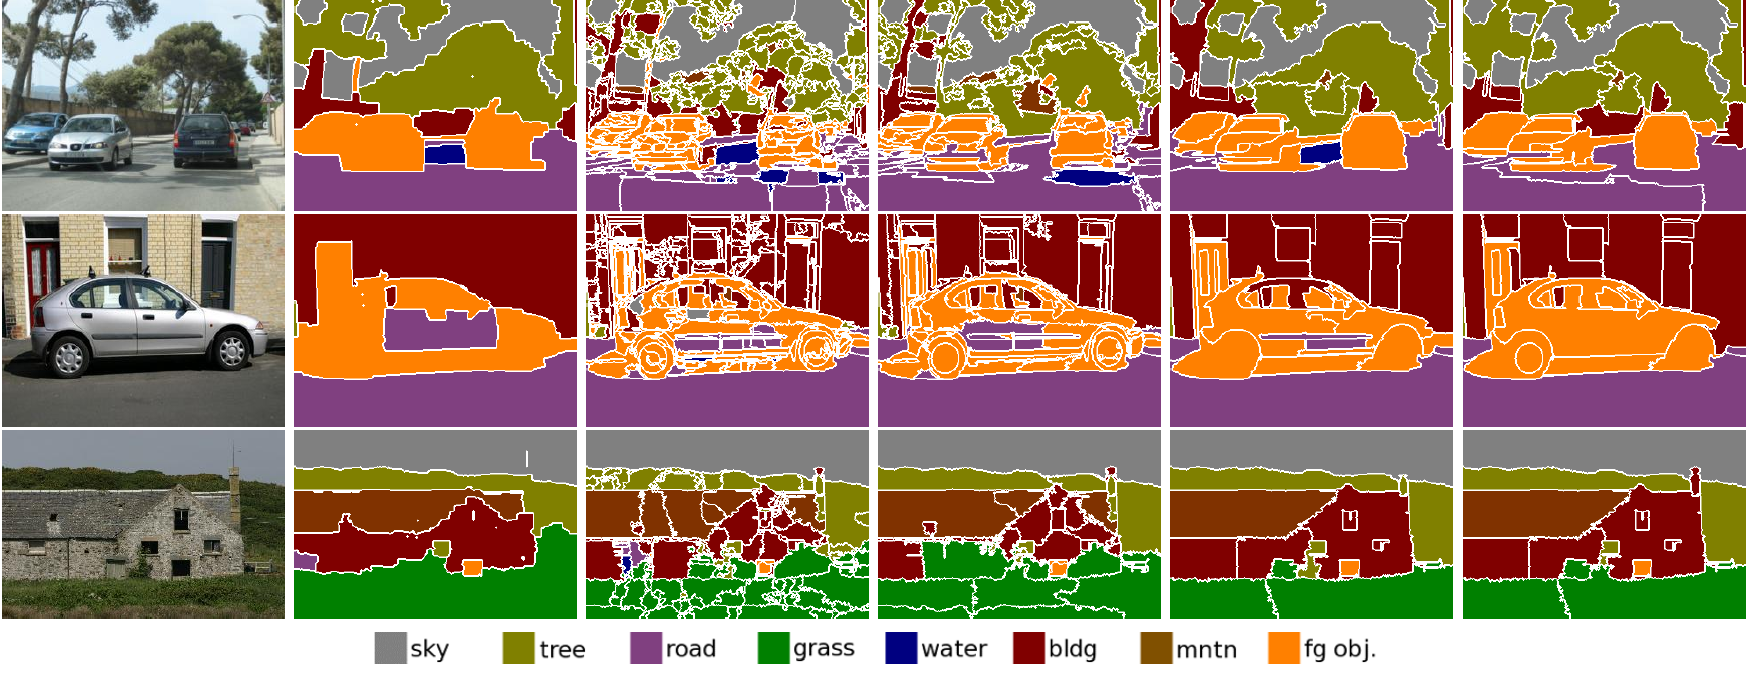
\includegraphics[width=0.9\textwidth]{L5F1.png}
        \vspace{-10pt}
    \end{center}
    \caption{Comparison of region segmentation algorithms based on object classification. Notice that regions are completely separated from each other by boundaries.}
\end{figure}

\section{Definition of Segmentation}
Formally, an image I is partitioned into $N$ regions if it satisfies the following properties:

\begin{itemize}
    \item $R_1 \cup R_2 \cup R_3 ... R_{N-1} \cup  R_N = I$
    \item $R_i \cap R_j = \phi, i \ne j$
\end{itemize}
\noindent
As we are segmenting the image by color, we need predicates (constraints) to determine the extent of regions. To simplify the discussion, let's begin by assuming out images are greyscale. Some examples of  predicates are:

\begin{itemize}
    \item All pixels in a region must have the same intensity.
    \item All pixels in a region must be within a set intensity interval.
    \item The standard deviation of intensities in a region must be less than a certain value
\end{itemize}

\section{Thresholds and Histograms}
When the image only contains one object, let's say a grey block on a black tablecloth, the greyscale image is a split into two regions. One region (the object) is represented by some intensity value, while the other (background) is represented by a different intensity value. When we plot the pixel intensities on a histogram, we see two peaks. Thus to get the two regions, we can define a single threshold $T$ in between the two peaks of the histogram to segment the image. This special type of thresholding results in a \textbf{binary image}.  

\begin{figure}[!htb]
    \begin{center}
        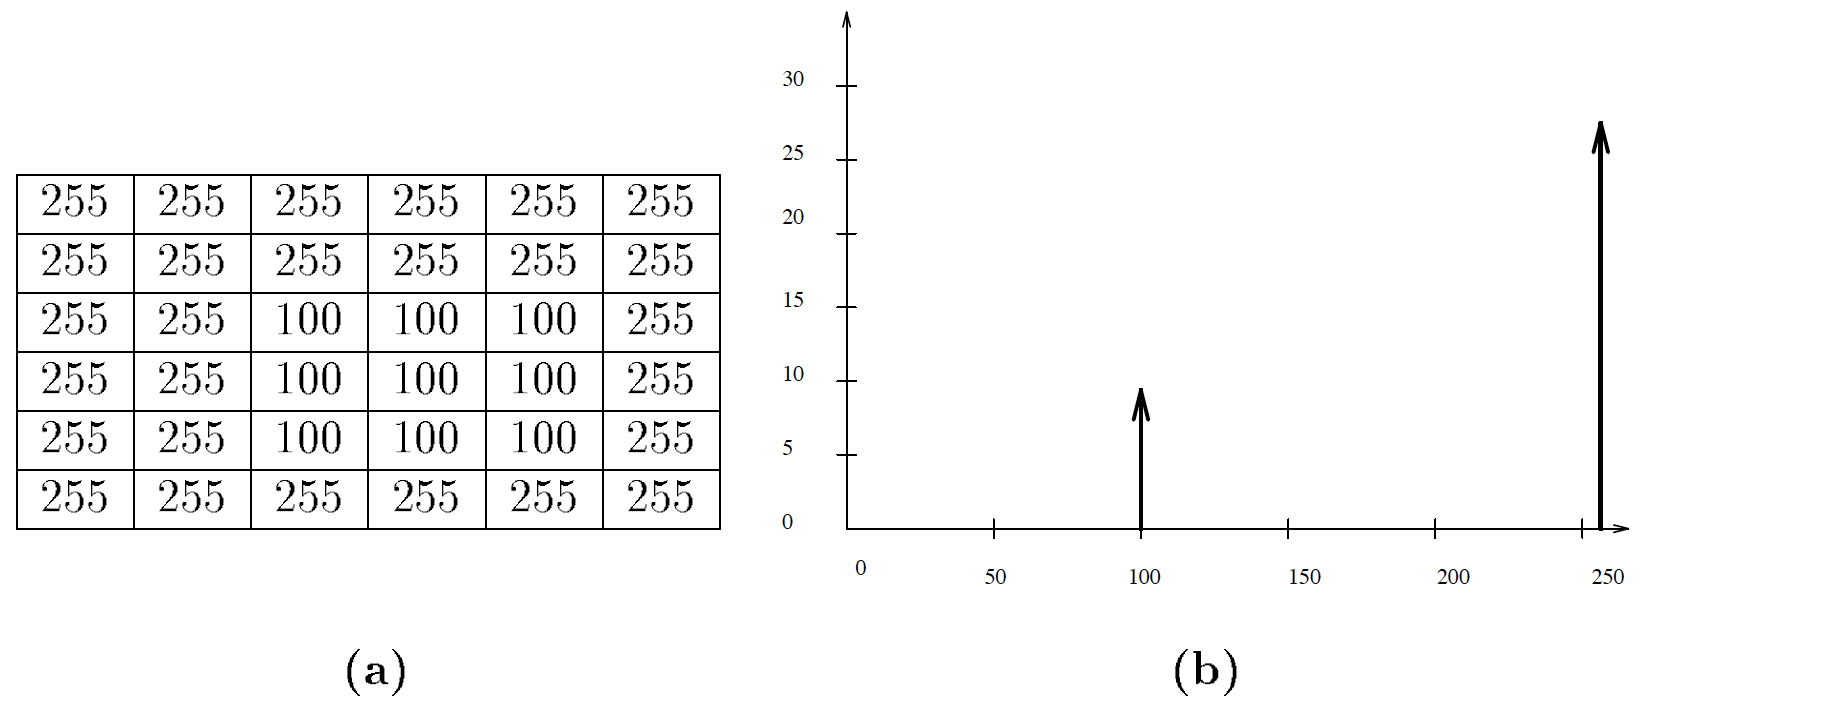
\includegraphics[width=0.9\textwidth]{L5F2.png}
        \vspace{-20pt}
    \end{center}
    \caption{(a) binary image, (b) histogram}
\end{figure}
\noindent

$$
J(x, y) = \left\{
        \begin{array}{ll}
            1 \quad \text{if} \quad I(x, y) > T \\
            0 \quad \text{otherwise}
        \end{array}
    \right.
$$

\noindent
Notice that binary images can contain more than two regions (e.g. many identical objects on a background). For images that cannot be segmented into a binary image, the pixel intensity of the segmented image, $J(x, y)$, depends on the relation of the corresponding pixel intensity in the original image, $I(x, y)$, to a range of thresholds. 

We can decompose the image into a histogram of color intensities and choose thresholds at the valleys of the histogram (remember in a histogram we can count the number of pixels in each interval) to obtain the regions. If there are $N$ regions, there are $N-1$ thresholds, and we end up with $N$ binary images, where the region of interest is represented by an intensity of 1 while everything else 0. From these images, we can assign each region a label and build a complete segmented image.

\begin{figure}[!htb]
    \begin{center}
        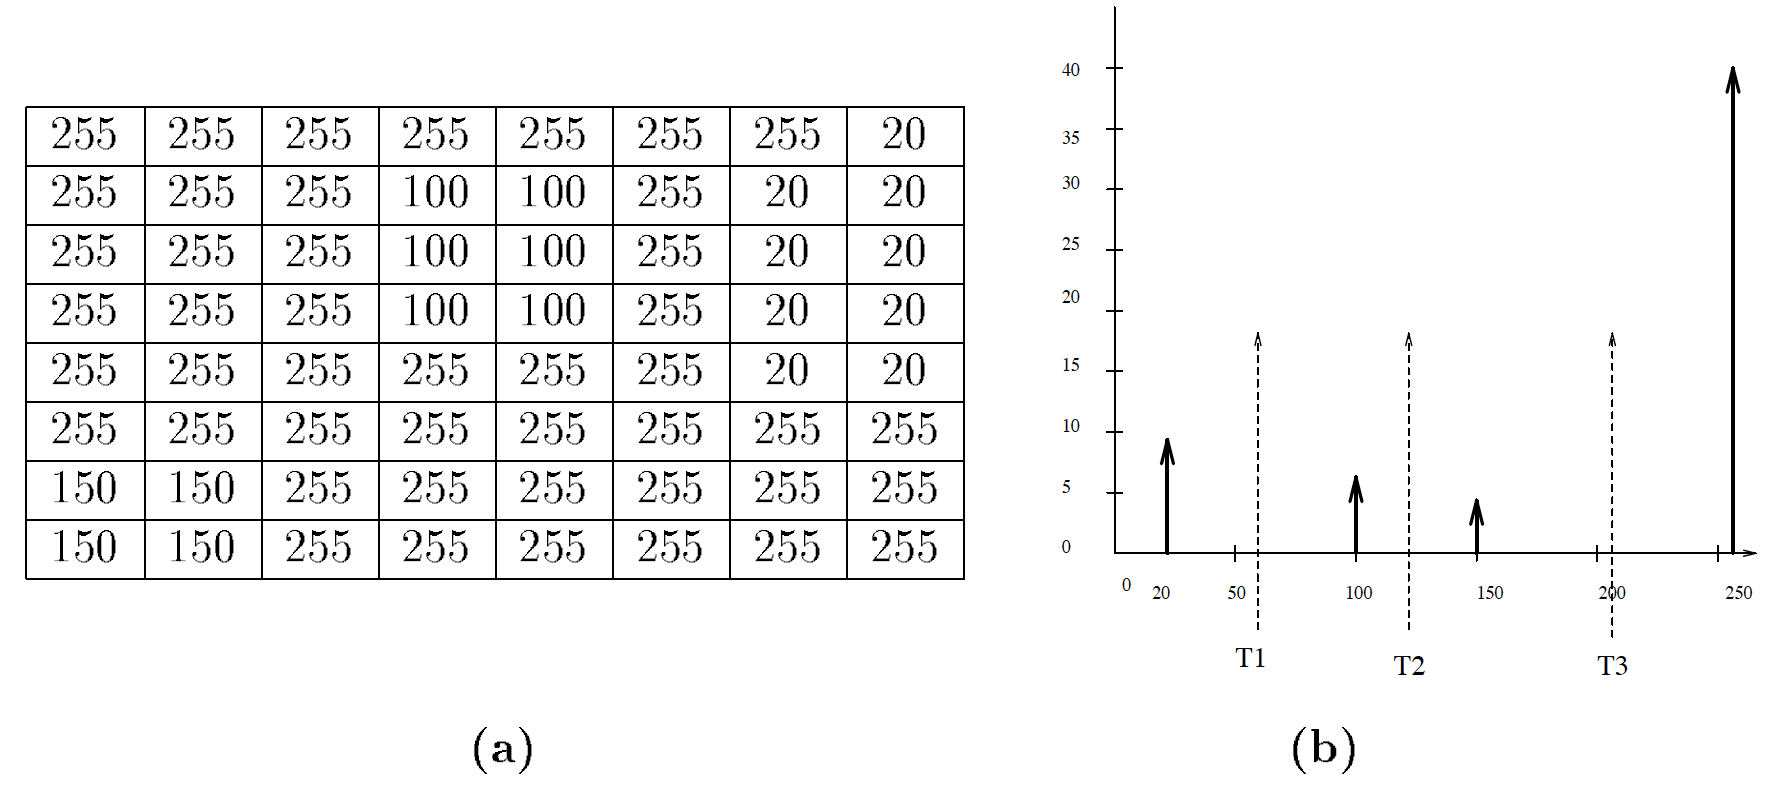
\includegraphics[width=0.9\textwidth]{L5F3.png}
        \vspace{-20pt}
    \end{center}
    \caption{(a) image with multiple regions, (b) histogram}
\end{figure}
\noindent

\section{Peakiness Test}
Real life images are not discrete. They contain are contain a continuous spectrum of pixel intensities and noise. Thus the peaks of the histogram are not discrete. The \textbf{Peakiness Tests} decides which peaks in the histogram actually represent objects and thus regions. Good peaks are sharp and tall. The test is based on the following characteristics of a peak.

\begin{itemize}
    \item $W$, $P$ = width, height of peak
    \item $V_a$, $V_b$ = height of two valleys on side of the peak
    \item $N$ = number of pixels under peak (peak area)
\end{itemize}

\noindent
The sharpness of a peak is defined as the ratio of the area of the peak to the rectangle formed by its width and height: $\frac{N}{W * P}$. Tall peaks are measured by the ratio of peak height to the average height of the adjacent valleys: $\frac{V_a+V_b}{2*P}$. The peakiness is defined as a product of these factors. If the peakiness is greater than some threshold, then the peak will be used for segmentation.

$$ Peakiness = (1-\frac{N}{W * P}) * (1-\frac{V_a+V_b}{2*P})$$

\begin{figure}[!htb]
    \begin{center}
        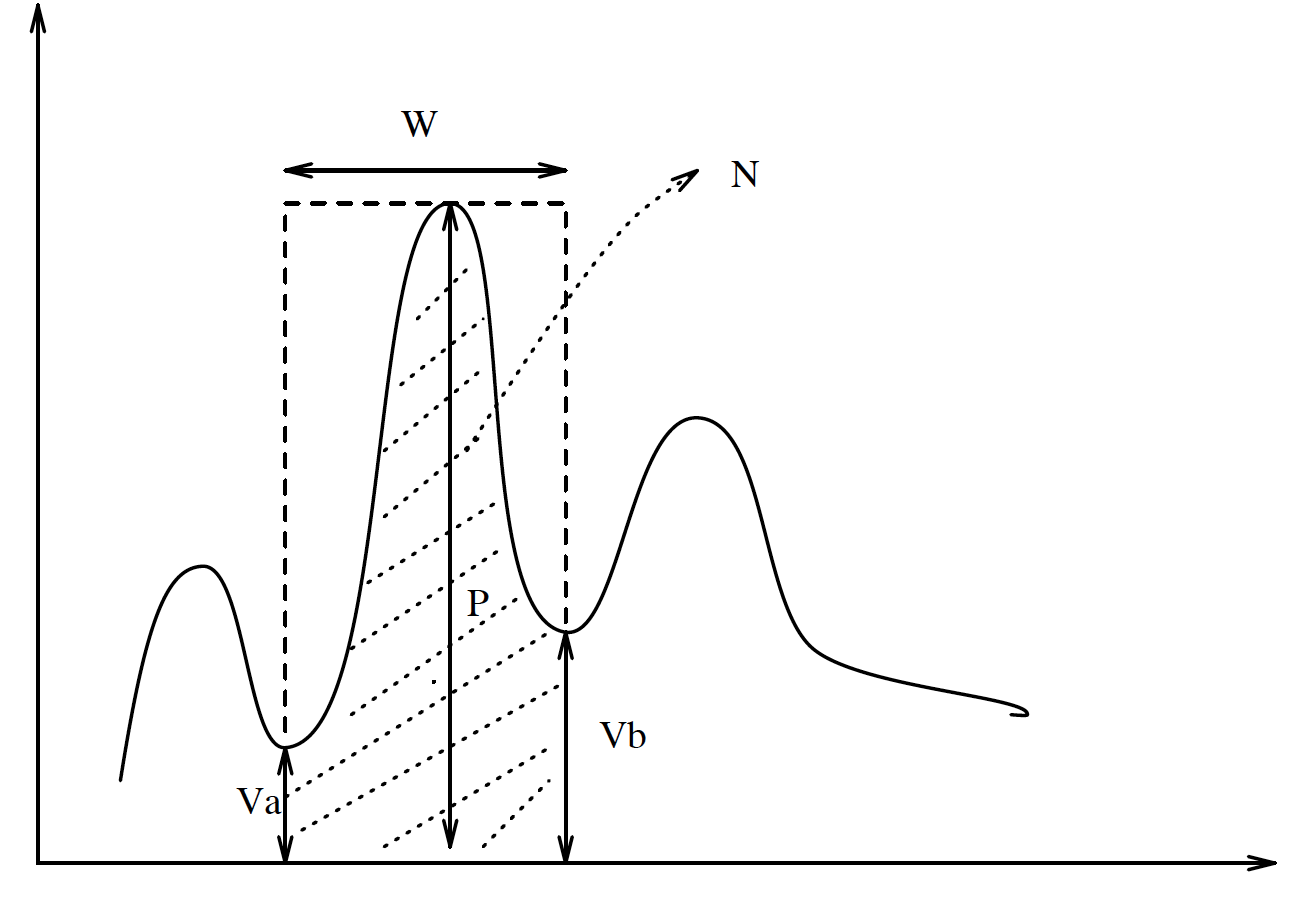
\includegraphics[height=4cm,width=0.5\textwidth]{L5F4.png}
        \vspace{-20pt}
    \end{center}
    \caption{Components of a Histogram Peak}
\end{figure}

\noindent
\section{Connected Components}
We $N$ regions and $N$ binary images, so how do we combine them into one image? Notice that we can process the binary images over a sliding window of time, meaning at the first instance, we segment the image based on the first threshold, and the at the second instance, the first and second thresholds, so on... and at the last instance, the last threshold. Let's assign each instance of time an id, and apply the sliding window. Every time we apply the thresholding, we also perform flood fill on the image (setting pixels in region to be 1), and then assign all 1 pixels the id. The end result is a fully segmented image. This algorithm runs in $O(N*P)$, where $P$ is the number of pixels.

\begin{figure}[!htb]
    \begin{center}
        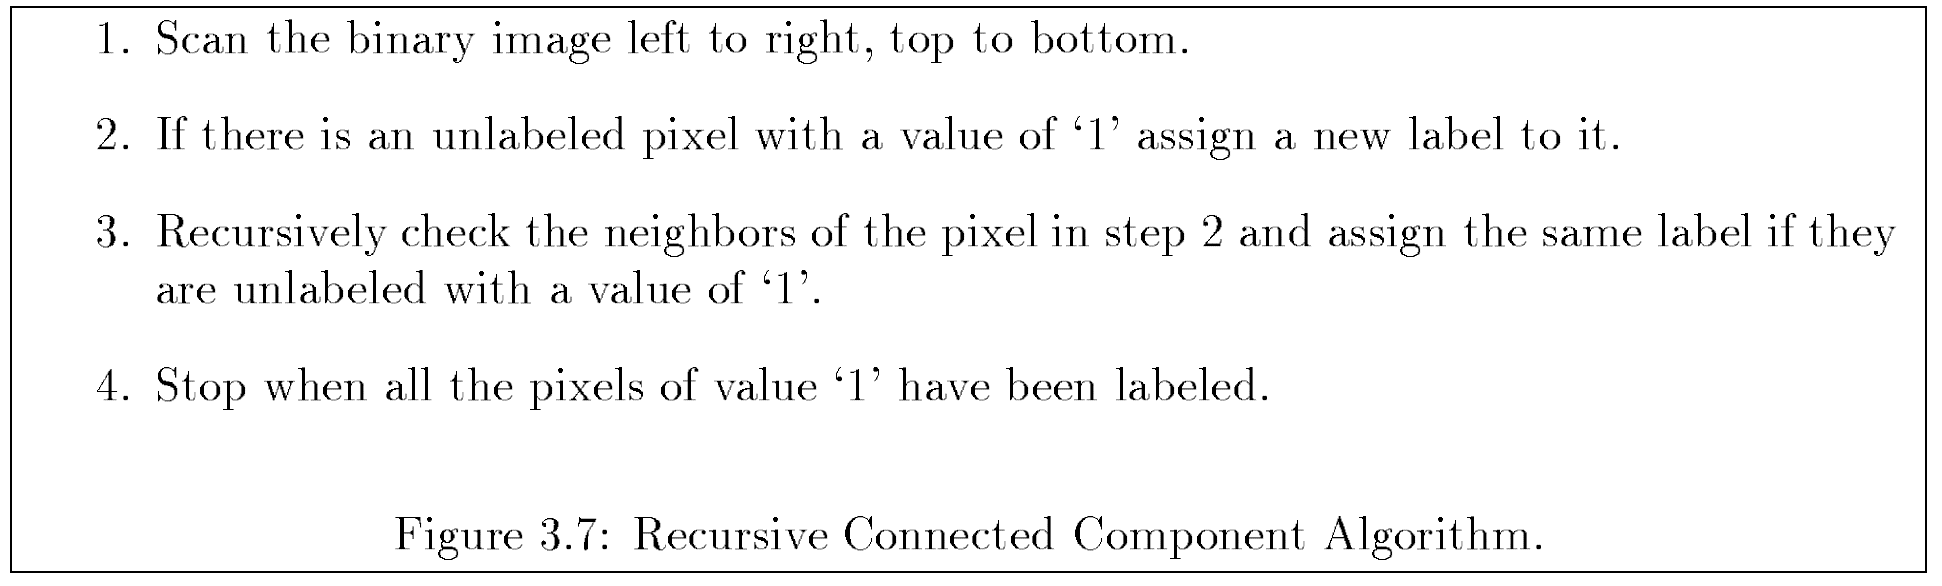
\includegraphics[width=0.7\textwidth]{L5F5.png}
        \vspace{-20pt}
    \end{center}
    \caption{Recursive Algorithm}
\end{figure}

\noindent
\noindent
The issue with a recursive algorithm is that we are constrained by the memory of the call stack. We can also apply a two-pass sequential algorithm. This algorithm is based on \textbf{equivalence classes}, which is like an id of a region. Let's assume in a binary image we have two regions. If we suddenly find a connection, then then we set the regions' equivalence classes equal to each other. In the end, we reassign regions with equivalent equivalence classes to a master equivalence class. 

\begin{figure}[!htb]
    \begin{center}
        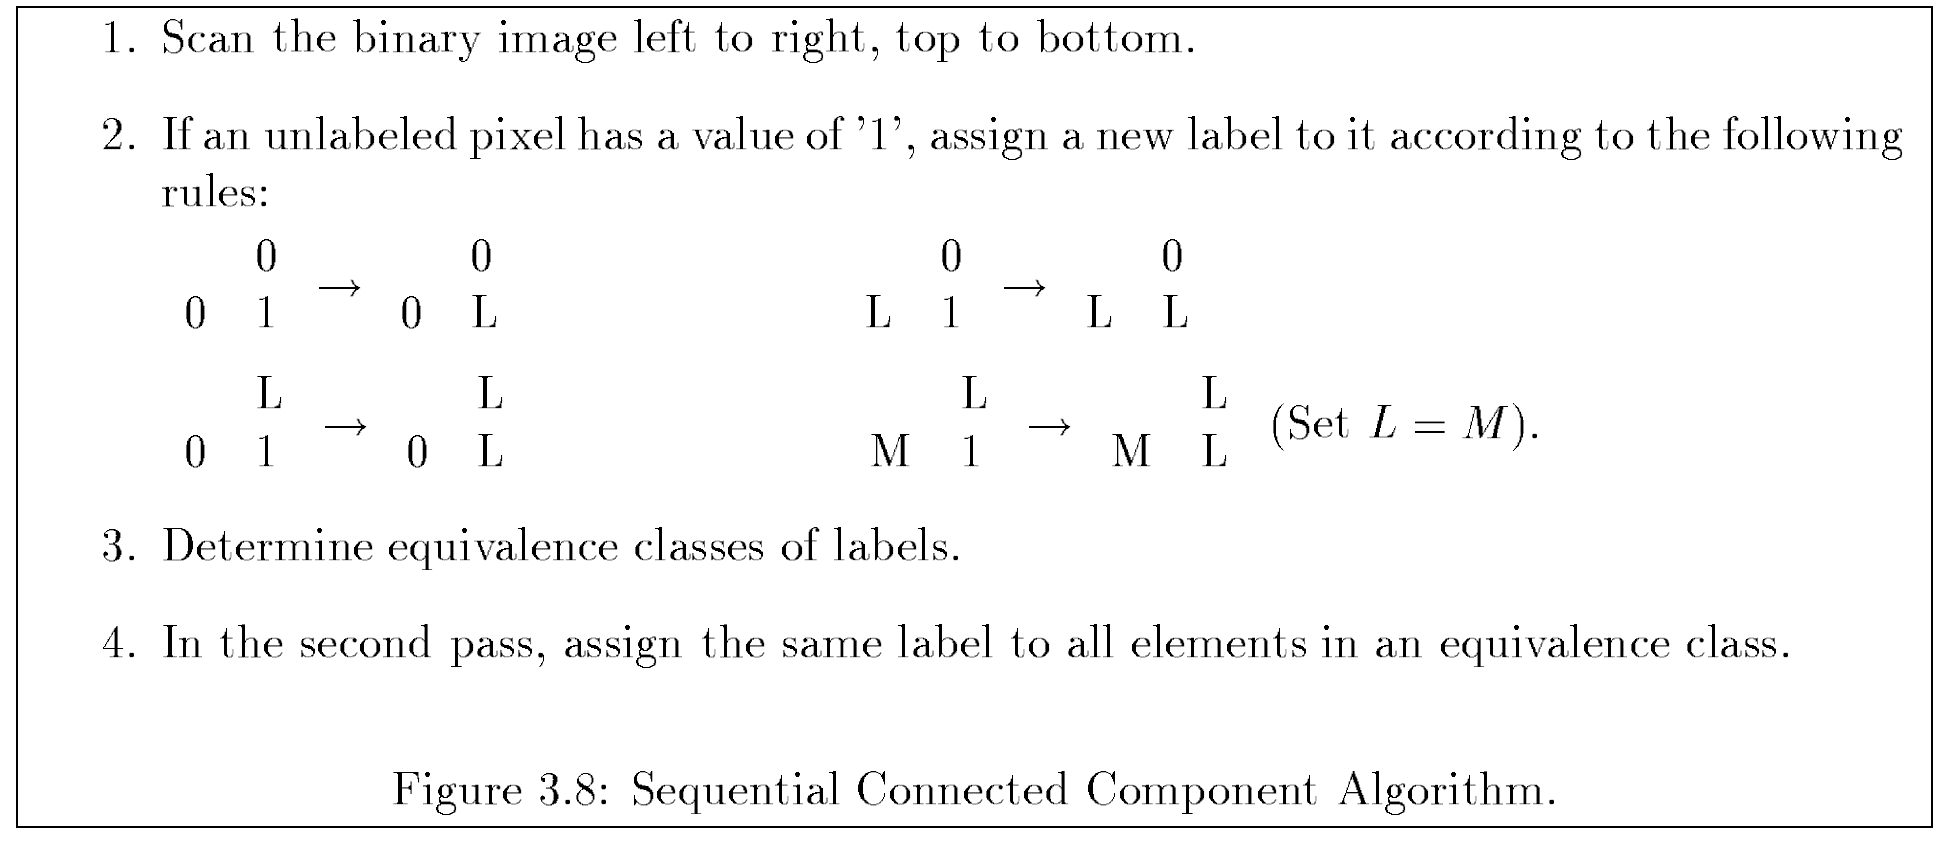
\includegraphics[width=0.7\textwidth]{L5F6.png}
        \vspace{-20pt}
    \end{center}
    \caption{Sequential Algorithm}
\end{figure}

\noindent
The final image segmentation algorithm is presented below:

\begin{figure}[!htb]
    \begin{center}
        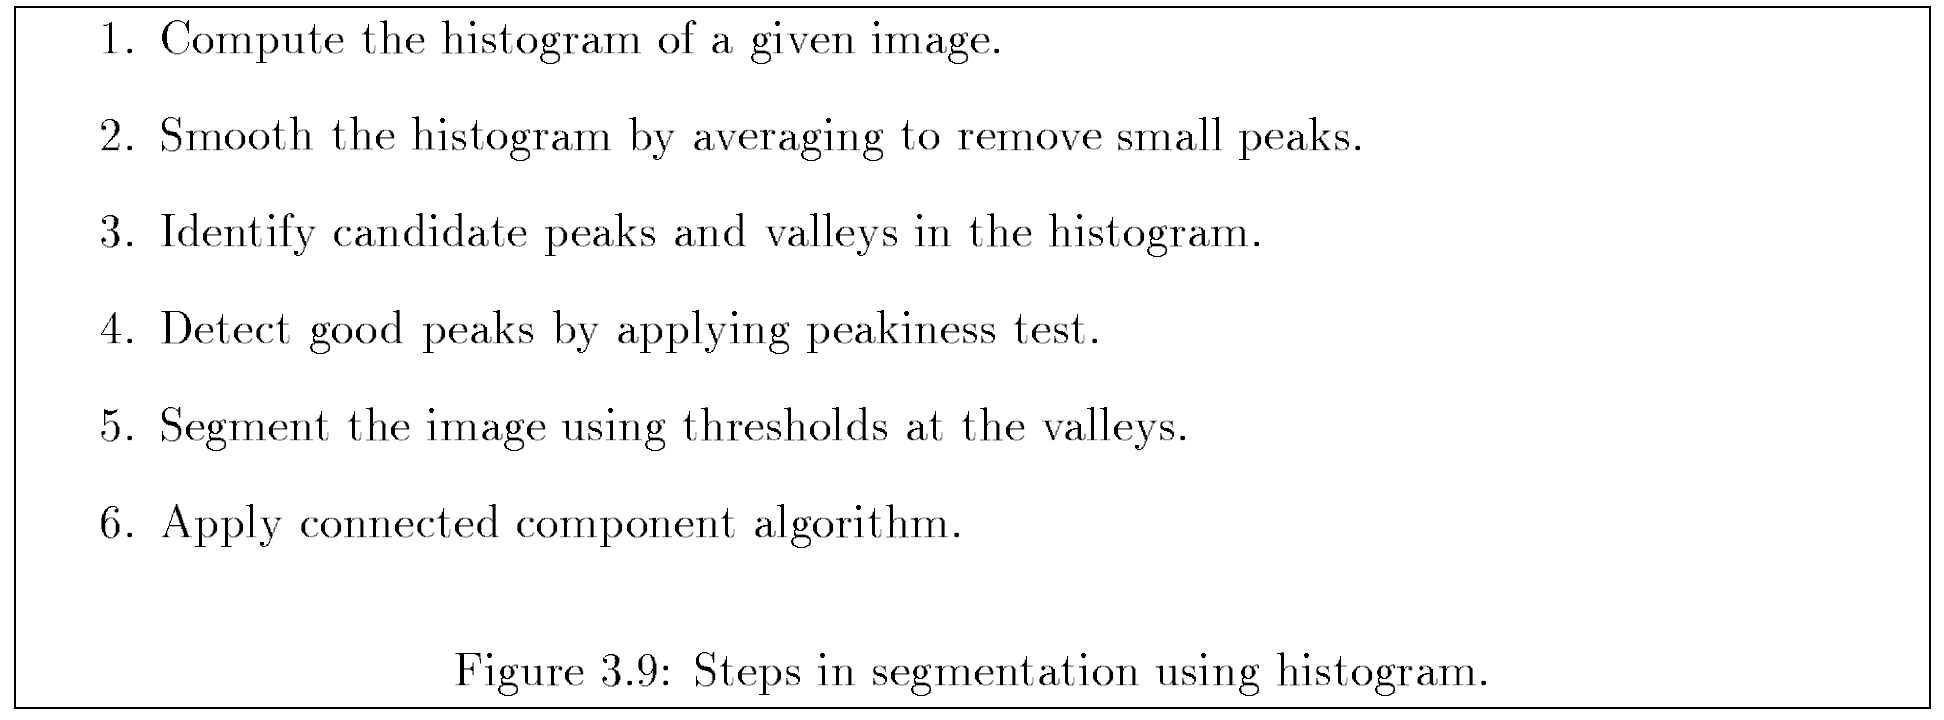
\includegraphics[width=0.7\textwidth]{L5F7.png}
        \vspace{-20pt}
    \end{center}
    \caption{Image segmentation Algorithm}
\end{figure}

\noindent

\section{Region Growing}
Often image segmentation yields too many regions (see Figure 1) that we want to merge into larger, more representative regions. Imagine we have the initial segmented image, or \textbf{seed segmentation}. We can refine it through region growing algorithms.

The simplest region growing algorithm is \textbf{split and merge}. We have a predicate (e.g. same pixel intensity) that determines if two regions are merged or split. There are also a lot of other region growing algorithms, and many of them involve \textbf{graph theory}.

\begin{figure}[!htb]
    \begin{center}
        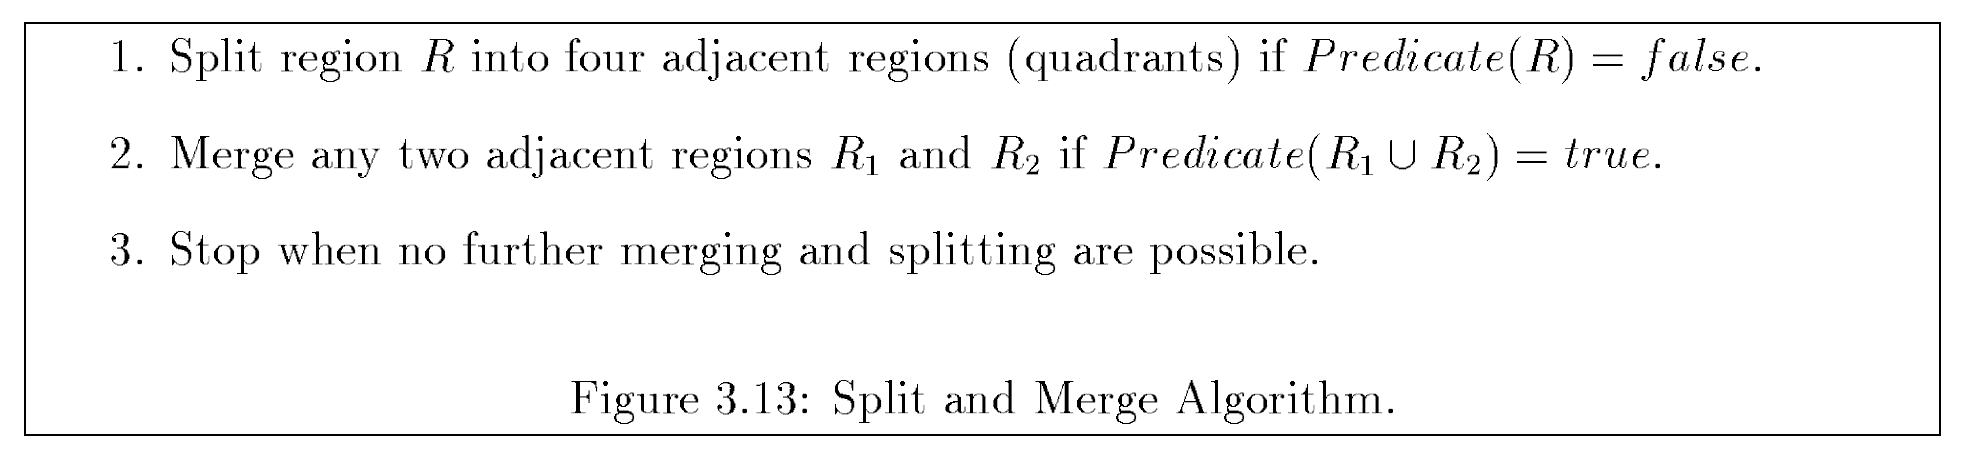
\includegraphics[width=0.7\textwidth]{L5F8.png}
        \vspace{-20pt}
    \end{center}
    \caption{Split Merge Algorithm}
\end{figure}

\begin{figure}[!htb]
    \begin{center}
        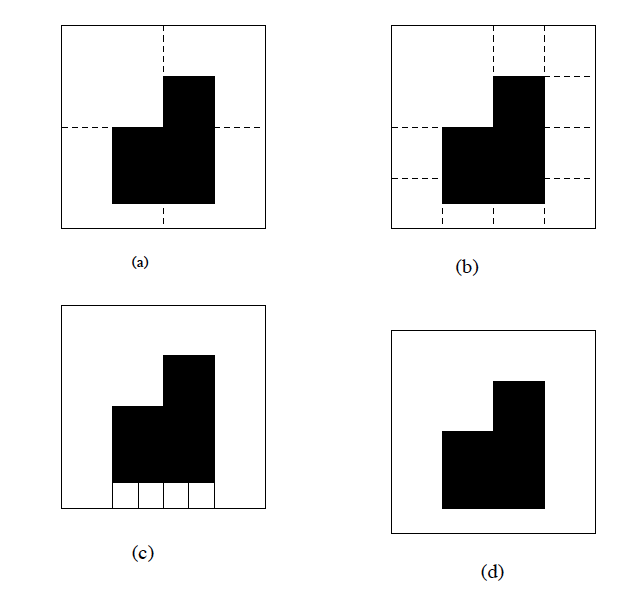
\includegraphics[width=0.7\textwidth]{L5F9.png}
        \vspace{-20pt}
    \end{center}
    \caption{Demonstration of the Split Merge Algorithm}
\end{figure}

\begin{figure}[!htb]
    \begin{center}
        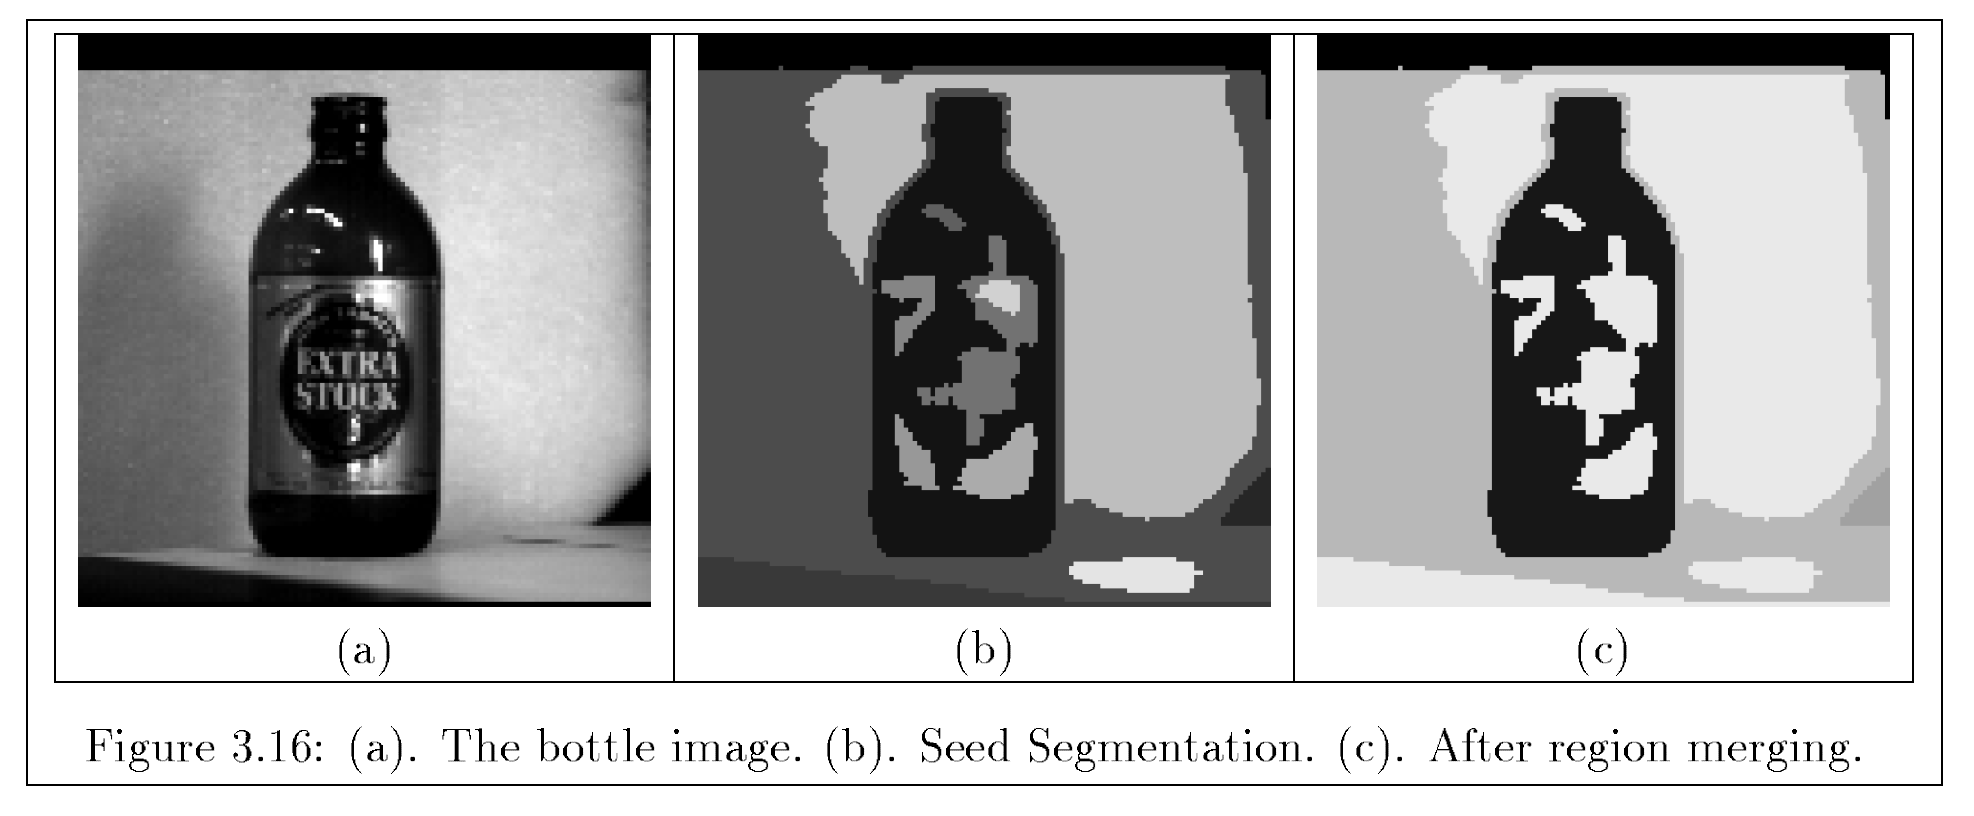
\includegraphics[width=0.7\textwidth]{L5F10.png}
        \vspace{-20pt}
    \end{center}
    \caption{Entire Image Segmentation Process}
\end{figure}

\section{Applications}
The applications of image segmentation are numerous. First, because image segmentation divides the image into different regions with similar properties, it can aid in locating objects and classify objects. In traffic control systems or autonomous vehicles, it can help pinpoint objects in the surroundings. In the medical field, image segmentation allows doctors to see different areas of the body and observe blood flow.

In this lecture we covered only the basics of image segmentation. Modern segmentation is usually accomplished using convolutional neural networks or robust computer vision algorithms, but many of the concepts are the same.
\end{document}
